% !TeX root = ../../../main.tex
\subsection{Sensitivity Analyses}
\label{ch05:apd:sensitivity-analyses}



\ChFiveHeadingOnly
\subsubsection{Sensitivity to Parts of the LLM Prompt Being Changed}
\label{ch05:apd:sensitivity-llm-prompt}

We slightly modified the prompt from the preceding section to check for sensitivity to specific parts of the LLM prompt being removed or modified.
This led to the following variants:
\begin{enumerate}\raggedright
    \item \textbf{No changes}: Original LLM query prompt. %
    
    \item \textbf{No role:} Remove the initial sentence \texttt{"You are a physician."}
    
    \item \textbf{Zero-shot prompting:} Remove the example case report and textual time series from the prompt. \\
    \textcolor{teal}{\texttt{An 18-year-old male was admitted to ...}}\\
    "Let's find the locations of events in the case report, it shows that ... then the output should look like:"\\
    \texttt{18 years old | 0 \\
    male | 0 \\
    ..}

    \item \textbf{No conjunction expansion:} Remove the following sentence from the prompt: \texttt{"Separate conjunctive phrases into their component events and assign them the same timestamp (for example, separation of ‘fever and rash’ into 2 events: ‘fever’ and ‘rash’)"}
    
    \item \textbf{Interval:} A query was added to the prompt for extracting the time interval (start and end time of clinical events).
The original prompt’s instructions and few-shot examples were modified accordingly. 
    
    \item \textbf{Interval + Type:} A query was added to the prompt for extracting the time interval and i2b2
    event type (Interval+Type), where event type is one of: Factual, Possible, Hypothetical, Conditional, Negated, Historical, Uncertain.
The original prompt’s instructions and few-shot examples were modified accordingly. 
\end{enumerate}


\ChFiveParagraph{Semantic similarity:}
The cumulative distributions of cosine distances between predicted and reference event phrases show clear differences across prompt variants. \emph{Interval} and \emph{Interval+Type} produce the closest matches, while \emph{Zero-shot} performs substantially worse, with a right-shifted distribution indicating lower-quality event spans. \emph{No role} and \emph{No conjunction} show modest degradation relative to the full prompt.
These results
demonstrate that including structured temporal guidance and explicit event formatting improves semantic alignment.

\ChFiveParagraph{Temporal ordering.}
The concordance index (c-index) follows a similar pattern. \emph{Interval+Type} achieves the highest median concordance, followed by \emph{Interval} and the full prompt.
Removing role
framing or conjunction splitting reduces ordering consistency, and \emph{Zero-shot} again yields the lowest performance with greater variability.
This suggests that structured instructions help the model maintain coherent temporal ordering among extracted events.

\ChFiveParagraph{Timestamp accuracy.}
Overall log-time discrepancy curves show that \emph{Interval} and \emph{Interval+Type} provide the most accurate timestamp predictions, whereas \emph{Zero-shot} exhibits the largest errors.
When stratified by temporal distance from presentation, prompt differences are minimal for
immediate events but widen substantially at longer horizons (1~day, 1~week, 1~year, and beyond).
Structured prompts with explicit temporal cues maintain accuracy across these
intervals, while unstructured prompts degrade more quickly.

When stratified by the time from presentation (e.g., within 1 hour, 1 day, 1 week), prompt differences are most pronounced for events occurring farther from the report anchor (Figure \ref{ch05:fig:prompt_ablation}, far right).
For immediate events, all prompt versions perform comparably.
However, at longer timescales (1 week to "ever"), Interval and Interval+Type maintain superior accuracy, while Zero-shot shows dramatic drops in performance.
This suggests that structured prompts are particularly critical for accurate long-range temporal reasoning.

Across semantic similarity, temporal ordering, and timestamp alignment, prompt components that provide explicit temporal structure or event-typing requirements consistently improve
performance, while removing instructional scaffolding—particularly in the Zero-shot condition—results in substantial degradation.
These findings highlight the importance of prompt
design in guiding LLMs to produce high-quality temporal annotations from clinical narratives.


\subsubsection{Inter-LLM Comparison of Temporal Annotations} 
\label{ch05:apd:inter-llm-comparison}

To illustrate qualitative differences among annotators, we compare temporal event sequences generated by several LLMs for a representative case report (PMC10629858) \citep{abu2023rare}, which describes a patient with lepromatous leprosy who later developed abdominal complications, recurrent bacteremia, severe sepsis, and ultimately died (Figure~\ref{ch05:fig:compare_llm_annotations}).


% !TeX root = ../../../main.tex
\begin{ChFiveUncaptionedFigure}
\begin{ChFiveFloatBody}
  \centering
    \begin{tcolorbox}[colback=white,colframe=black!30,boxrule=0.6pt,left=2mm,right=2mm,top=2mm,bottom=2mm,width=\linewidth]
    \footnotesize \textbf{Excerpt from \cite{abu2023rare}:}
    \begin{quote}\footnotesize
    A 57-year-old man recently diagnosed with lepromatous leprosy was confirmed with skin biopsy and had been on treatment (rifampicin/clofazimine/dapsone) for 2 months before admission; he was presented to the hospital with complaints of abdominal distension, constipation, vomiting, and a 10-kg weight loss. On examination, the patient was vitally stable. He had evidence of peripheral lymphadenopathy with a distended abdomen and a positive shifting dullness. A computed tomography scan of his abdomen showed mural thickening of the terminal ileum with significantly enlarged mesenteric lymph nodes, mesenteric fat stranding, and intra-abdominal free fluid, suggesting abdominal granulomatous infection or neoplastic process.
    \dots 
    
    The patient was planned for consolidation by autologous bone marrow transplant. Unfortunately, with the recurrent bacteremia and sepsis that accompanied the patient’s course due to his immunocompromised state, he was re-admitted to the medical ICU for severe sepsis and multiorgan failure and passed away around 6 months after his initial diagnosis with NHL, despite maintaining a remission status.
    \end{quote}
    \end{tcolorbox}
  \begin{minipage}[t]{0.45\linewidth}\centering
    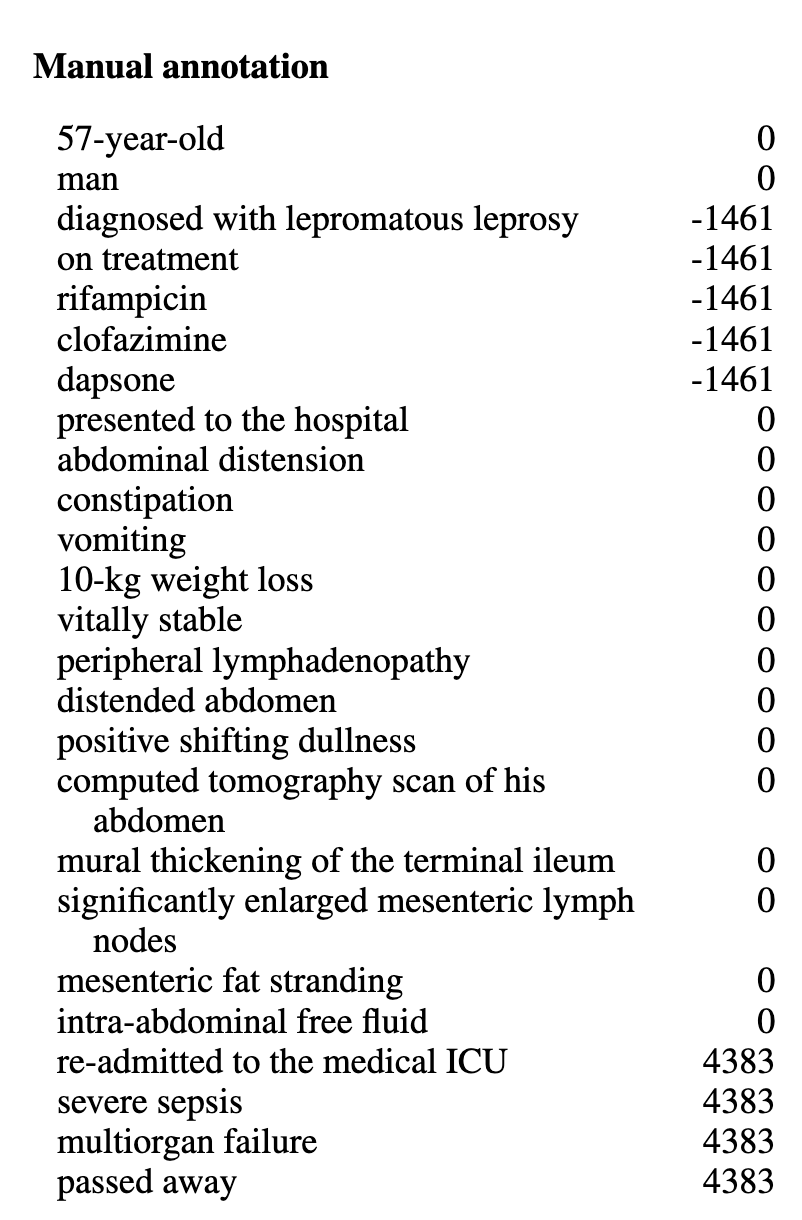
\includegraphics[width=0.9\linewidth]{Appendices/appendix-ch05/images/Scientific_data/Supplementary/example_TTS_for_paper/manual.png}
  \end{minipage}\hfill
  \begin{minipage}[t]{0.45\linewidth}\centering
    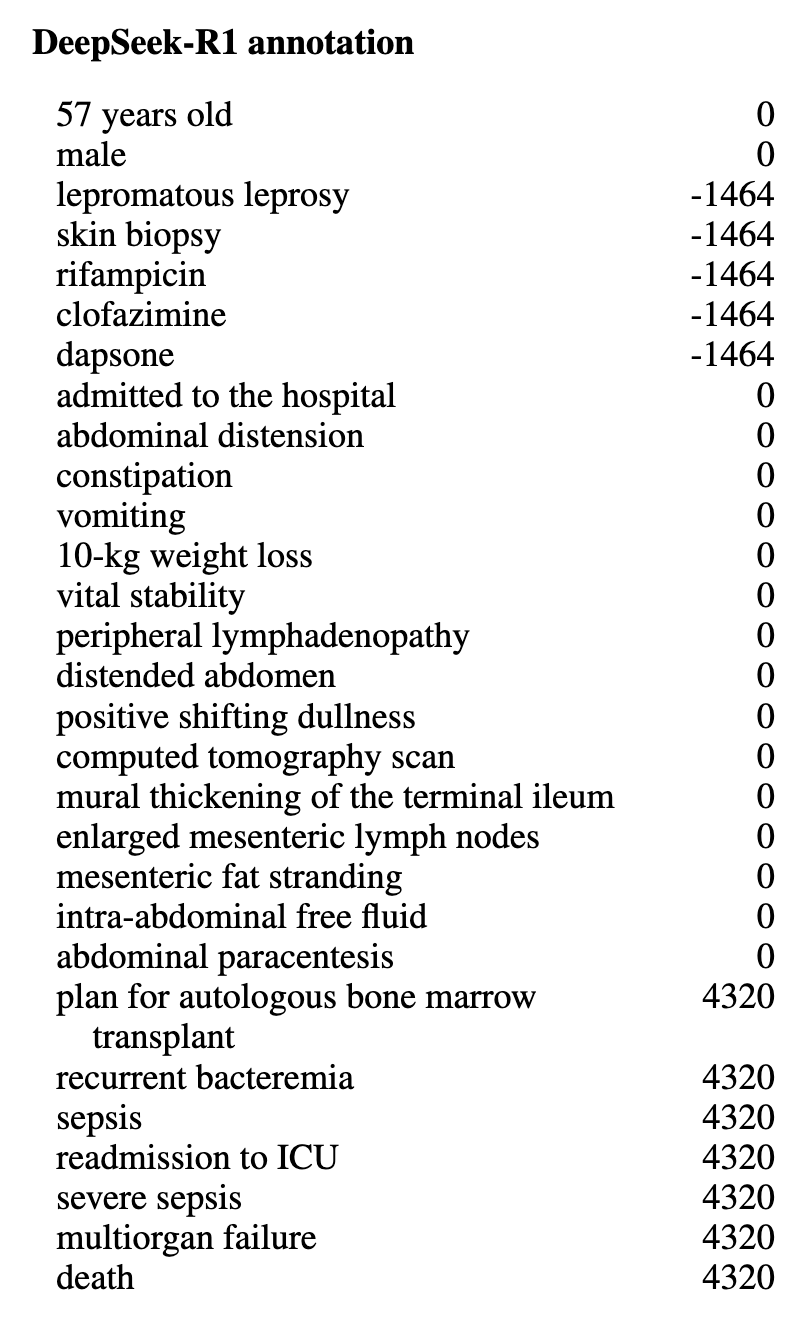
\includegraphics[width=0.9\linewidth]{Appendices/appendix-ch05/images/Scientific_data/Supplementary/example_TTS_for_paper/DeepSeekR1.png}
  \end{minipage}


  \begin{minipage}[t]{0.45\linewidth}\centering
    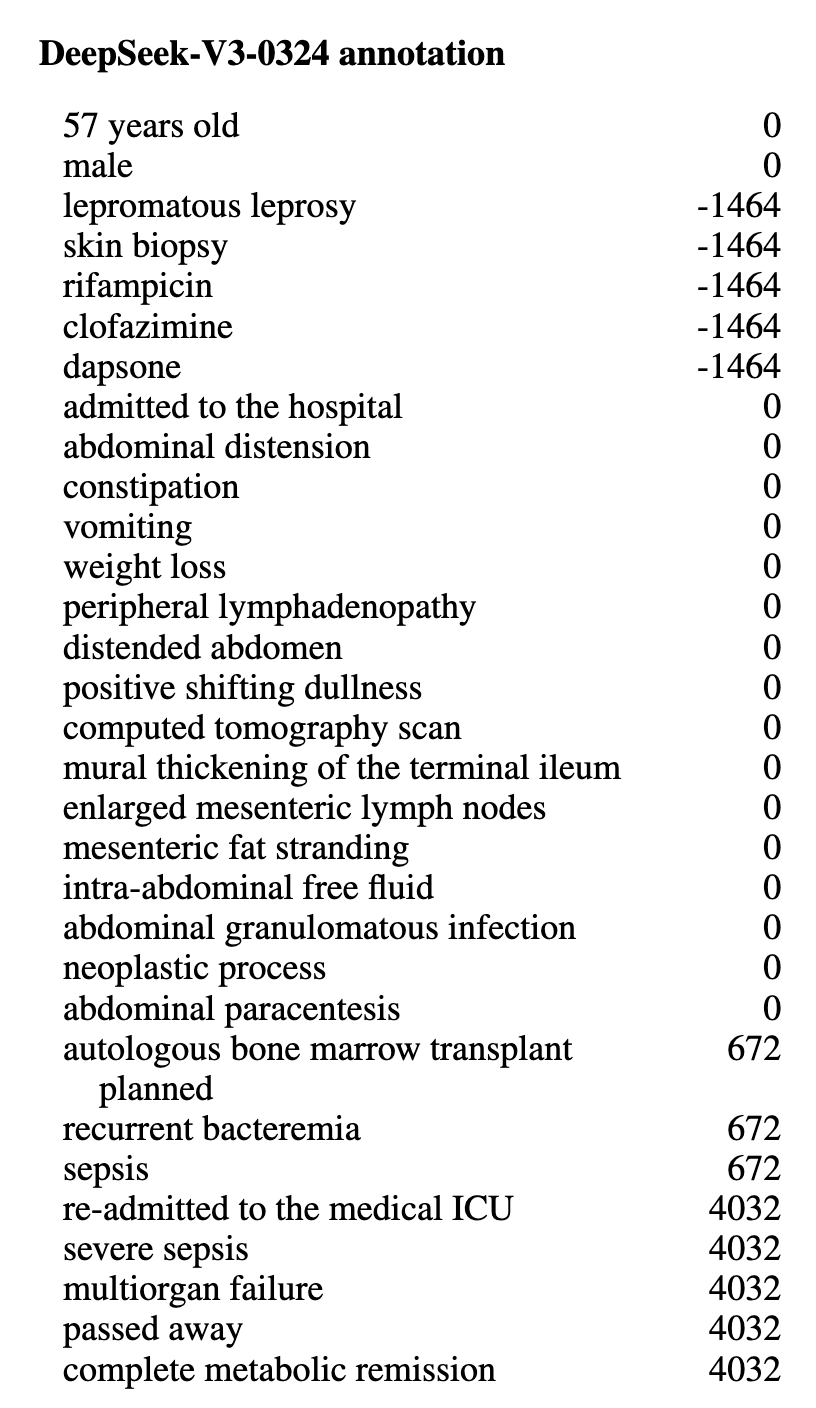
\includegraphics[width=0.9\linewidth]{Appendices/appendix-ch05/images/Scientific_data/Supplementary/example_TTS_for_paper/DeepSeekV3.png}
  \end{minipage}\hfill
  \begin{minipage}[t]{0.45\linewidth}\centering
    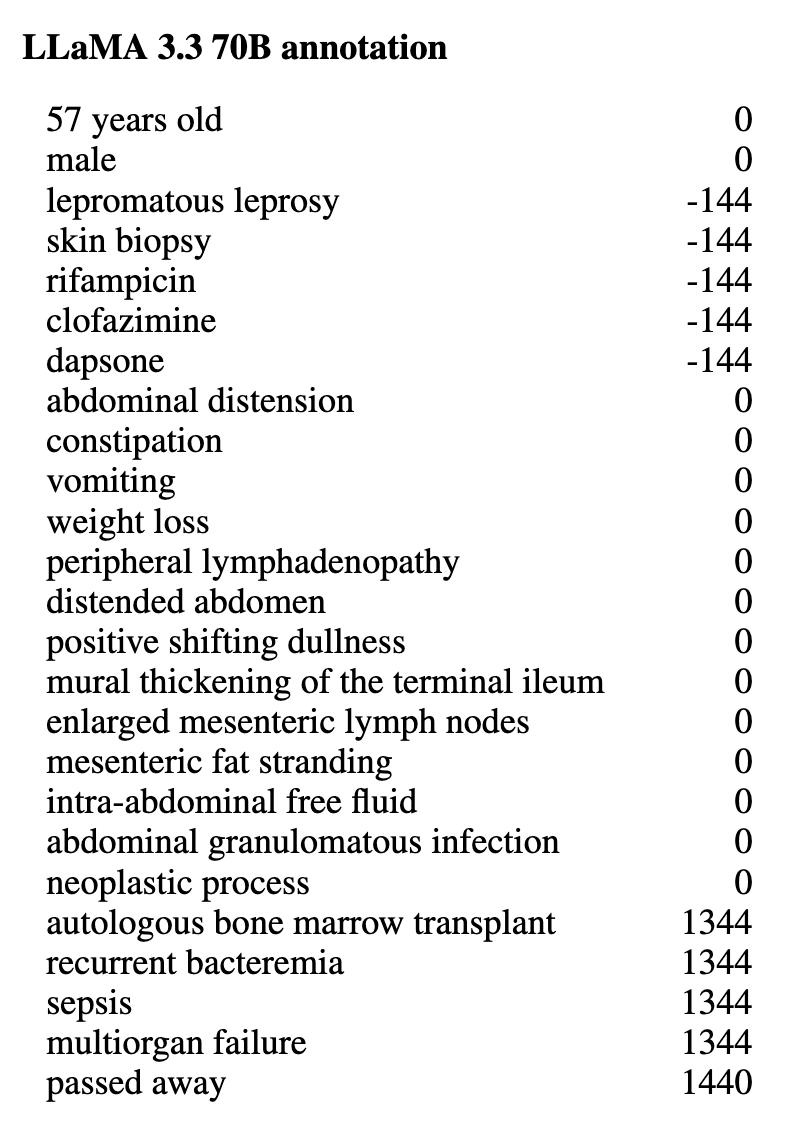
\includegraphics[width=0.9\linewidth]{Appendices/appendix-ch05/images/Scientific_data/Supplementary/example_TTS_for_paper/L3370B.png}
  \end{minipage}

\end{ChFiveFloatBody}
\end{ChFiveUncaptionedFigure}




% !TeX root = ../../../main.tex
\begin{figure}[htbp]
\begin{ChFiveFloatBody}

  \centering
  \begin{minipage}[t]{0.45\linewidth}\centering
    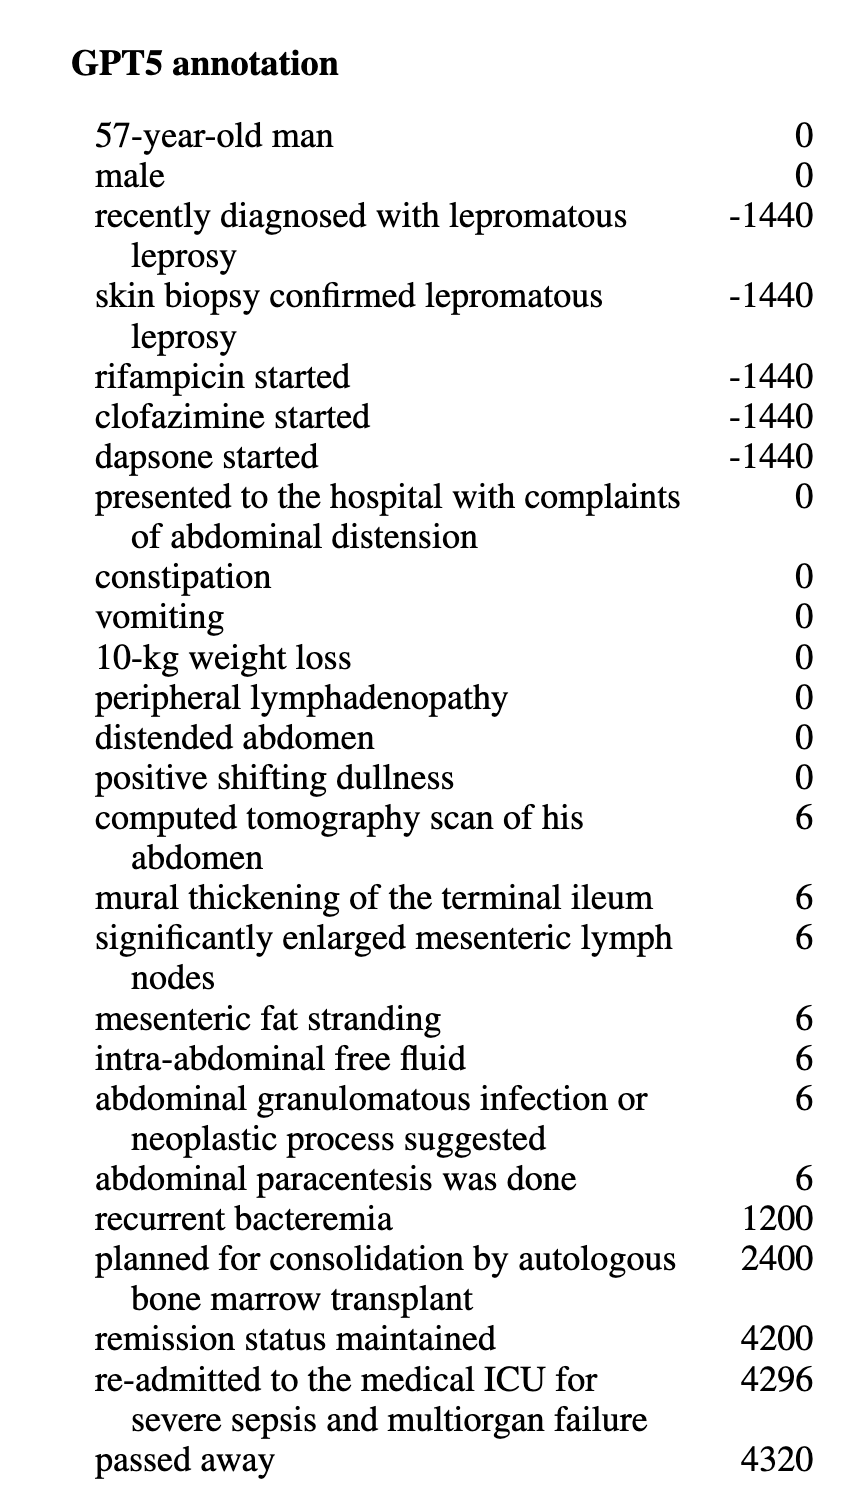
\includegraphics[width=0.9\linewidth]{Appendices/appendix-ch05/images/Scientific_data/Supplementary/example_TTS_for_paper/GPT5.png}
  \end{minipage}\hfill
  \begin{minipage}[t]{0.45\linewidth}\centering
    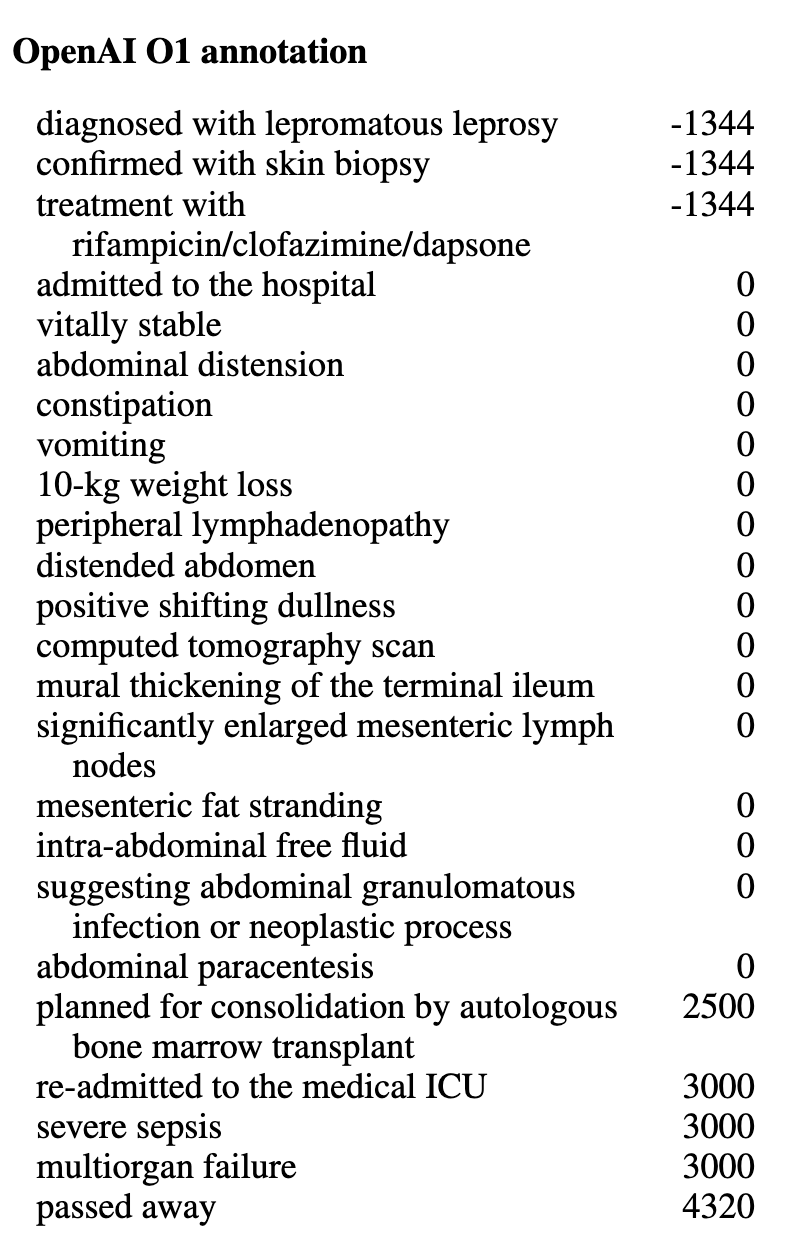
\includegraphics[width=0.9\linewidth]{Appendices/appendix-ch05/images/Scientific_data/Supplementary/example_TTS_for_paper/O1.png}
  \end{minipage}

  

  \begin{minipage}[t]{0.45\linewidth}\centering
    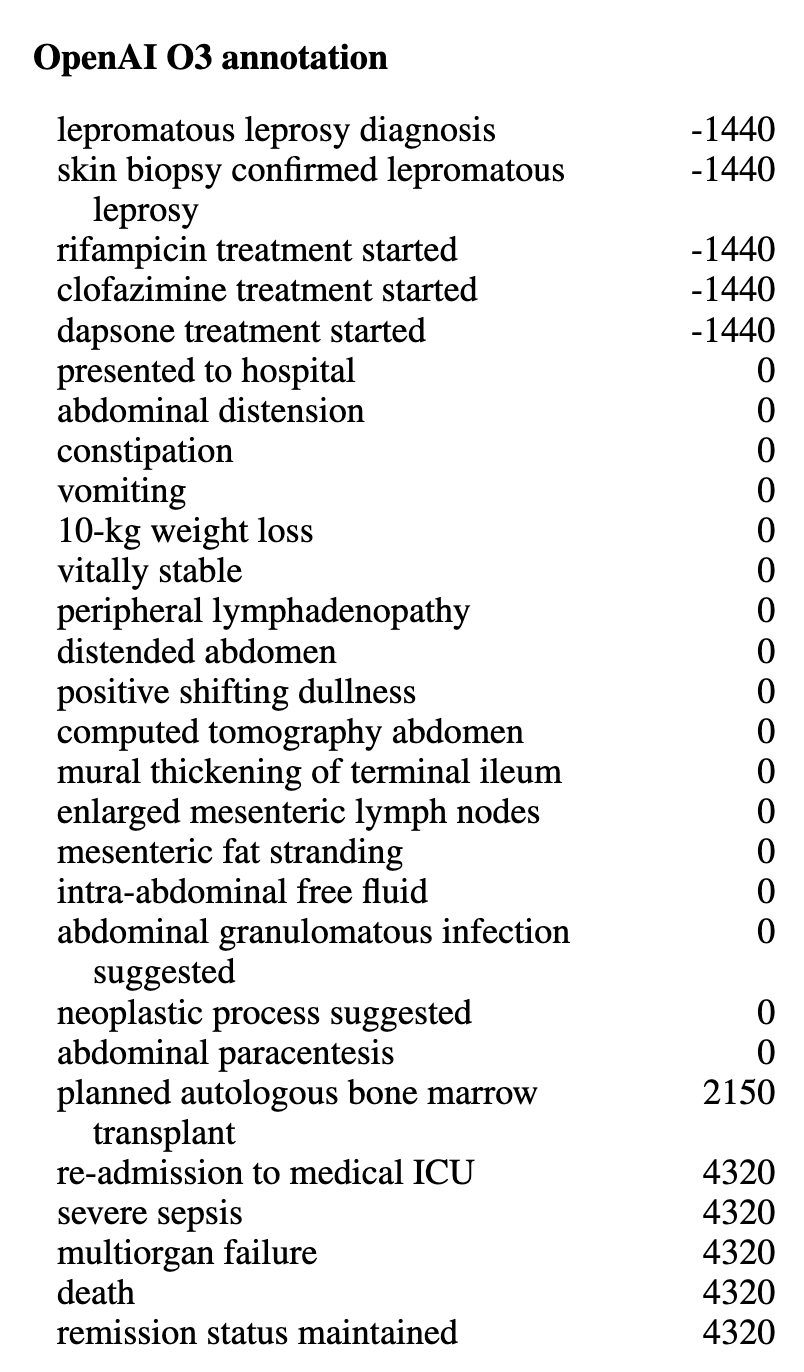
\includegraphics[width=0.9\linewidth]{Appendices/appendix-ch05/images/Scientific_data/Supplementary/example_TTS_for_paper/O3.png}
  \end{minipage}\hfill
  \begin{minipage}[t]{0.45\linewidth}\centering
    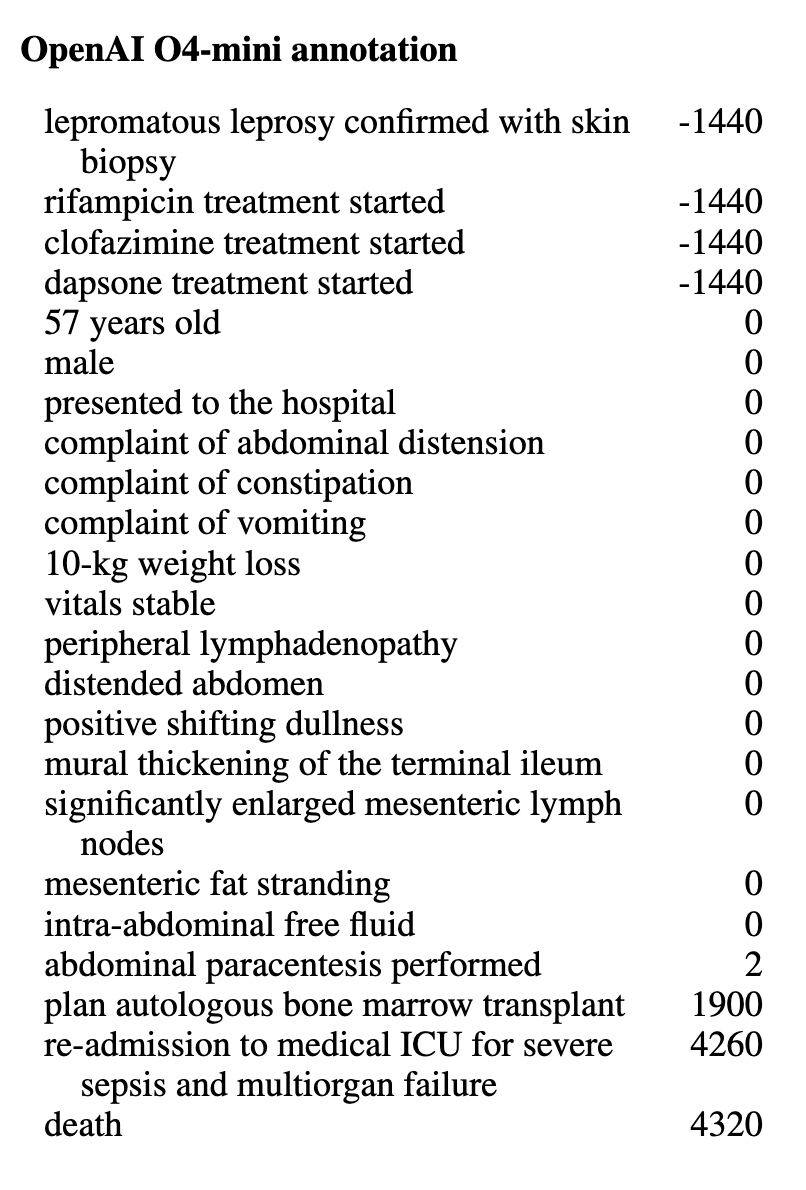
\includegraphics[width=0.9\linewidth]{Appendices/appendix-ch05/images/Scientific_data/Supplementary/example_TTS_for_paper/O4mini.png}
  \end{minipage}


  
  

\end{ChFiveFloatBody}
\caption{Comparison of temporal annotations generated by several LLMs for a representative case report (PMC10629858). The figure contrasts manual annotations with model-generated event–time
sequences, highlighting differences in event granularity, phrasing, duplicate event generation, and temporal normalization (e.g., variation in converting narrative expressions such as ``two
months before admission’’ into hour offsets). Long-range timestamp assignments (e.g., for transplant planning, ICU readmission, and death) show the greatest variability across models, whereas the overall ordering of major clinical events is largely preserved. This example illustrates characteristic
differences in how LLMs interpret, segment, and temporally anchor clinical narratives.}\ChFiveFloatLabel{ch05:fig:compare_llm_annotations}
\end{figure}



















Across models, the principal clinical trajectory is consistently recovered: confirmation of lepromatous leprosy, antibiotic treatment, evolving abdominal symptoms with corresponding imaging findings, subsequent sepsis, ICU readmission, and death.
All annotators preserve the
temporal polarity of events, assigning negative times to historical information and positive times to post-admission findings.

Differences emerge in event granularity and phrasing.
Some models split conjunctive phrases into multiple events (e.g., listing each component medication separately), whereas others
compress them into single entries.
Several annotators also produce near-duplicate events at the same timestamp (e.g., both “diagnosed with lepromatous leprosy’’ and “skin biopsy confirmed’’), reflecting variation in how models segment clinically related information within the narrative.

More pronounced differences appear in temporal normalization.
For the expression “two months before admission,” models produce hour offsets ranging from approximately $-1464$ to $-1344$, and one model assigns $-144$ due to an apparent day–hour unit error.
Long-range events such as the autologous bone marrow transplant plan, ICU readmission, and death also receive timestamps that vary by hundreds of hours across annotators.
Despite this variability in absolute timing,
the relative ordering of major clinical milestones remains largely preserved.

A recurring issue across models involves distinguishing planned actions from events that actually occurred.
For example, most annotators correctly represent “planned autologous bone-marrow transplant’’ with an associated future timestamp, which is appropriate because planned interventions can be temporally located and may influence subsequent decision-making.
However, several models omit the word “planned,’’ converting the entry into “autologous
bone-marrow transplant’’ and thereby representing an intended but unperformed procedure as an event that occurred.
In such cases, the discrepancy arises from the event label rather than the timestamp itself, illustrating how small linguistic omissions can alter the extracted temporal semantics.

% !TeX root = ../../../main.tex
\begin{table}[htbp]
\caption{Common error types observed across LLM-generated temporal annotations.}\ChFiveFloatLabel{ch05:tab:error_taxonomy}
\ChFiveTableBodyStart
\begin{ChFiveFloatBody}

\centering


\begin{tabular}{>{\raggedright\arraybackslash}p{3.2cm} >{\raggedright\arraybackslash}p{9cm}}
\toprule
\textbf{Error Type} & \textbf{Description and Examples} \\
\midrule

\textbf{Event granularity mismatch} 
& Models differ in splitting vs.\ compressing multi-component statements. 
For example, medications may appear as three separate events (``rifampicin'', ``clofazimine'', ``dapsone'') or as one combined entry. \\[6pt]

\textbf{Near-duplicate events} 
& Multiple paraphrased versions of the same clinical concept assigned to the same timestamp, such as 
``diagnosed with lepromatous leprosy’’ and 
``skin biopsy confirmed lepromatous leprosy.’’ \\[6pt]

\textbf{Temporal normalization variability} 
& Large differences in converting narrative expressions (e.g., ``two months before admission’’) to numerical timestamps, with offsets ranging from $-1464$ to $-1344$ hours and occasional scaling errors (e.g., $-144$ hours). Long-range events (e.g., transplant plan, ICU readmission, death) also vary by hundreds of hours across models. \\[6pt]

\textbf{Intent vs.\ occurrence confusion} 
& Some models omit modality markers such as ``planned,'' converting intended future events into events marked as completed. 
The timestamp itself may be reasonable; the error lies in the event label. \\[6pt]

\textbf{Phrasing and specificity variation} 
& Models differ in the level of detail used in event descriptions.  
Some outputs retain clinically precise phrases (e.g., ``mural thickening of the terminal ileum’’), while others produce generic events (e.g., ``abdominal abnormality’’). \\[6pt]

\textbf{Long-range timestamp degradation} 
& Accuracy decreases for events far from the admission anchor, with larger dispersion in timestamp predictions for events weeks or months after presentation. \\
\bottomrule
\end{tabular}


\end{ChFiveFloatBody}
\end{table}


Overall, the models capture the broad sequence of events but differ in how they segment conjunctive statements, handle near-duplicates, and resolve absolute times—particularly for
long-range events.
A taxonomy of common annotation errors observed across models—including granularity differences, duplicate events, temporal normalization variability, and intent–occurrence misclassification—is summarized in Table~\ref{ch05:tab:error_taxonomy}.


\subsubsection{Sensitivity to Event Matching Strategy (LAPJV)}
\label{ch05:apd:lapjv-matching}
We additionally consider a globally optimal one-to-one event alignment based on the Linear Assignment Problem, solved using the Jonker--Volgenant (LAPJV) algorithm \citep{jonker1987shortest}.
We define a rectangular cost matrix whose entries are pairwise cosine distances between predicted and reference events.
To enforce the same distance thresholding used in the recursive heuristic, we assign a large penalty cost to pairs whose distance exceeds the threshold, effectively masking infeasible matches.
LAPJV then computes a minimum-cost assignment under these constraints, yielding a globally optimal one-to-one alignment between the two event sets.

To assess sensitivity to the event alignment procedure, we repeat the inter-LLM comparison using LAPJV-based matching at a cosine distance threshold of 0.1.
Table~\ref{ch05:tab:model_comparison_lapjv} reports event match rate, temporal concordance, and AULTC across five independent runs per model, and is directly comparable to the main-text results obtained using the recursive matching heuristic (Algorithm~\ref{ch05:alg:recursive_match}; Table~\ref{ch05:tab:model_comparison}).
\texttt{OpenAI GPT5} achieves the highest mean match rate (0.850 $\pm$ 0.006), indicating the most comprehensive coverage of manually annotated events. \texttt{OpenAI O3} attains the highest concordance (0.894 $\pm$ 0.004), and \texttt{OpenAI O4-mini} yields the highest AULTC (0.749 $\pm$ 0.003), reflecting strong timestamp alignment among matched events. Standard deviations are generally small across runs, suggesting stable behavior for a given model.







% !TeX root = ../../../main.tex
\begin{table}[htbp]
\caption{\ChFiveRebuttal{Inter-LLM comparison under LAPJV-based event matching (threshold = 0.1), evaluated on 200 manually annotated case reports across five runs per model.}}\ChFiveFloatLabel{ch05:tab:model_comparison_lapjv}
\ChFiveTableBodyStart
\begin{ChFiveFloatBody}


\footnotesize
\centering
\setlength{\tabcolsep}{3pt}


\begin{tabular}{lccccc}
\hline
\textbf{Model} &
\begin{tabular}{c}\textbf{Event Match}\\\textbf{Recall}\end{tabular} &
\begin{tabular}{c}\textbf{Event Match}\\\textbf{Precision}\end{tabular} &
\begin{tabular}{c}\textbf{Event Match}\\\textbf{F1}\end{tabular} &
\textbf{Concordance} &
\textbf{AULTC} \\
\hline
\texttt{Llama 3.3 70B}
& 0.676 $\pm$ 0.003
& 0.761 $\pm$ 0.036
& 0.715 $\pm$ 0.015
& 0.848 $\pm$ 0.003
& 0.720 $\pm$ 0.001 \\

\texttt{DeepSeek-R1}
& 0.750 $\pm$ 0.008
& 0.793 $\pm$ 0.006
& 0.771 $\pm$ 0.006
& 0.773 $\pm$ 0.007
& 0.727 $\pm$ 0.004 \\

\texttt{DeepSeek-V3}
& 0.764 $\pm$ 0.005
& 0.801 $\pm$ 0.005
& 0.782 $\pm$ 0.004
& 0.777 $\pm$ 0.009
& 0.730 $\pm$ 0.002 \\

\texttt{OpenAI GPT-5}
& \textbf{0.851 $\pm$ 0.006}
& 0.761 $\pm$ 0.007
& \textbf{0.803 $\pm$ 0.003}
& \textbf{0.903 $\pm$ 0.004}
& 0.722 $\pm$ 0.001 \\

\texttt{OpenAI O4-mini}
& 0.752 $\pm$ 0.019
& 0.818 $\pm$ 0.015
& 0.783 $\pm$ 0.017
& 0.845 $\pm$ 0.006
& \textbf{0.750 $\pm$ 0.002} \\

\texttt{OpenAI O3}
& 0.738 $\pm$ 0.003
& 0.842 $\pm$ 0.002
& 0.786 $\pm$ 0.002
& 0.900 $\pm$ 0.005
& 0.737 $\pm$ 0.003 \\

\texttt{OpenAI O1}
& 0.640 $\pm$ 0.007
& \textbf{0.878 $\pm$ 0.003}
& 0.740 $\pm$ 0.005
& 0.881 $\pm$ 0.003
& 0.731 $\pm$ 0.002 \\
\hline
\end{tabular}


\end{ChFiveFloatBody}
\end{table}



We further examine the trade-off between event match rate and temporal accuracy by sweeping
the LAPJV distance threshold from 0.01 to 0.50 in increments of 0.01. 
Figure~\ref{ch05:fig:threshold_tradeoff_LAPJV}
plots temporal concordance and AULTC as a function of event match rate, with the operating
point at threshold 0.1 highlighted.


% !TeX root = ../../../main.tex
\begin{figure}[htbp]
\begin{ChFiveFloatBody}

    \centering
    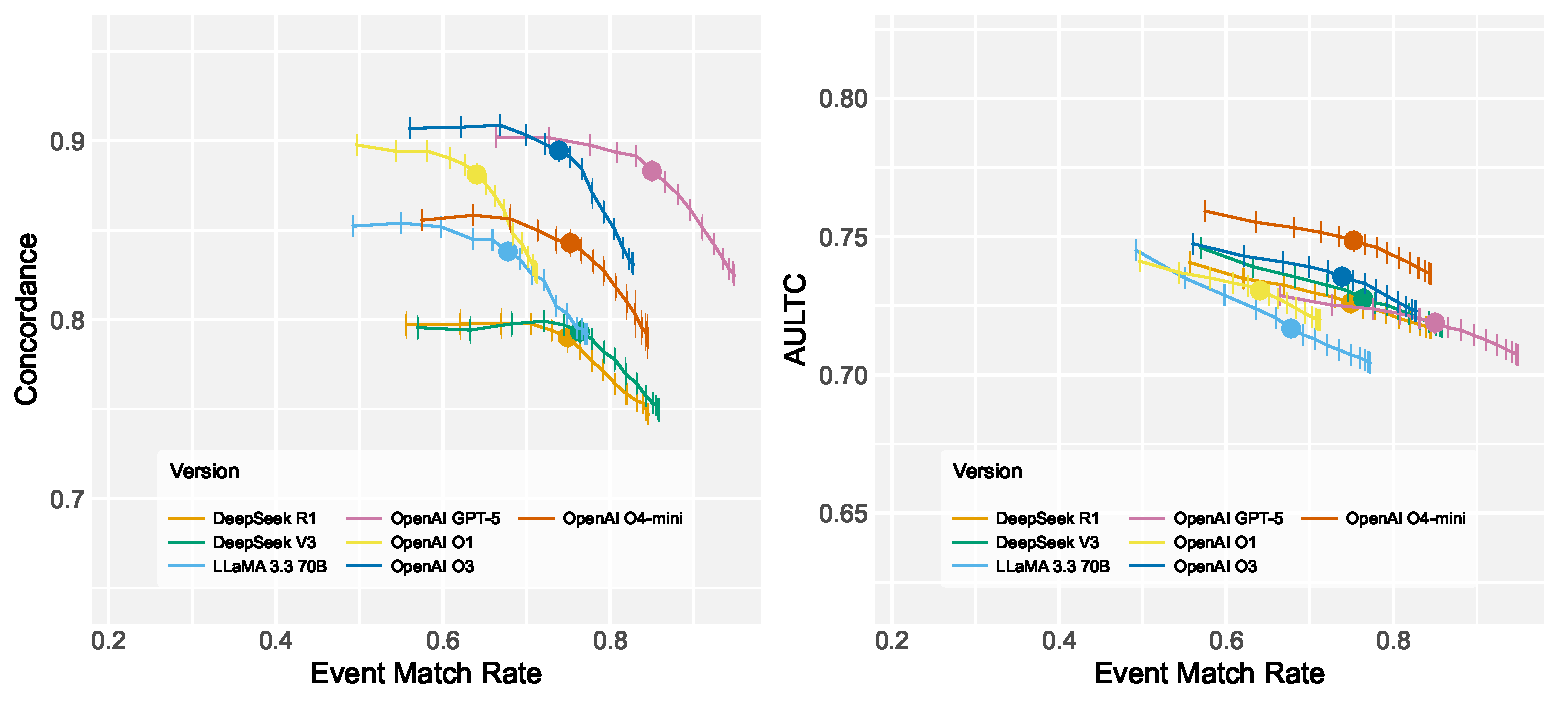
\includegraphics[width=\linewidth]{Appendices/appendix-ch05/images/Scientific_data/Plots_tables/event_match_vs_metrics_lapjv.pdf}
    
    
    

\end{ChFiveFloatBody}
\caption{\textbf{A:} Temporal concordance versus event match rate under LAPJV-based matching.
    \textbf{B:} AULTC versus event match rate. Solid circles ($\bullet$) indicate the operating
    threshold of 0.1; ticks (|) denote 0.01 threshold increments in [0.01, 0.50].}\ChFiveFloatLabel{ch05:fig:threshold_tradeoff_LAPJV}
\end{figure}


Across models, LAPJV preserves high event match rates at low thresholds and exhibits a
smooth trade-off between coverage and temporal accuracy. 
The resulting operating points in Figure~\ref{ch05:fig:threshold_tradeoff_LAPJV}
are highly comparable to those obtained using the recursive matching heuristic in Figure~\ref{ch05:fig:threshold_tradeoff_greedy} (e.g., at $\tau=0.1$, the operating point used in our main results in Table~\ref{ch05:tab:model_comparison}). 
In particular,
the heuristic matcher yields slightly stronger concordance near the elbow of the trade-off
curve, while LAPJV achieves marginally higher AULTC values, reflecting improved timestamp
alignment under global assignment. 
Overall, both strategies lead to consistent qualitative
conclusions.

















